% Architecture: ../poolformer.py, default PoolFormer-S12 at 224 x 224.
% Primary reference: https://github.com/sail-sg/poolformer/blob/main/models/poolformer.py
% Compile: pdflatex -halt-on-error poolformer.tex
% For an existing document, copy the color/style definitions and tikzpicture;
% load tikz with the arrows.meta library in that document's preamble.
\documentclass[tikz,border=8pt]{standalone}
\usepackage{amsmath}
\usetikzlibrary{arrows.meta}
\definecolor{poolblue}{HTML}{DCEAF7}
\definecolor{ink}{HTML}{24364B}
\tikzset{
  box/.style={draw=ink,rounded corners=3pt,thick,align=center,
    minimum height=22mm,text width=22mm,fill=poolblue},
  op/.style={box,minimum height=12mm,text width=16mm},
  sum/.style={draw=ink,circle,thick,minimum size=6mm,inner sep=0pt},
  flow/.style={-{Stealth[length=2mm]},thick,draw=ink}
}
\begin{document}
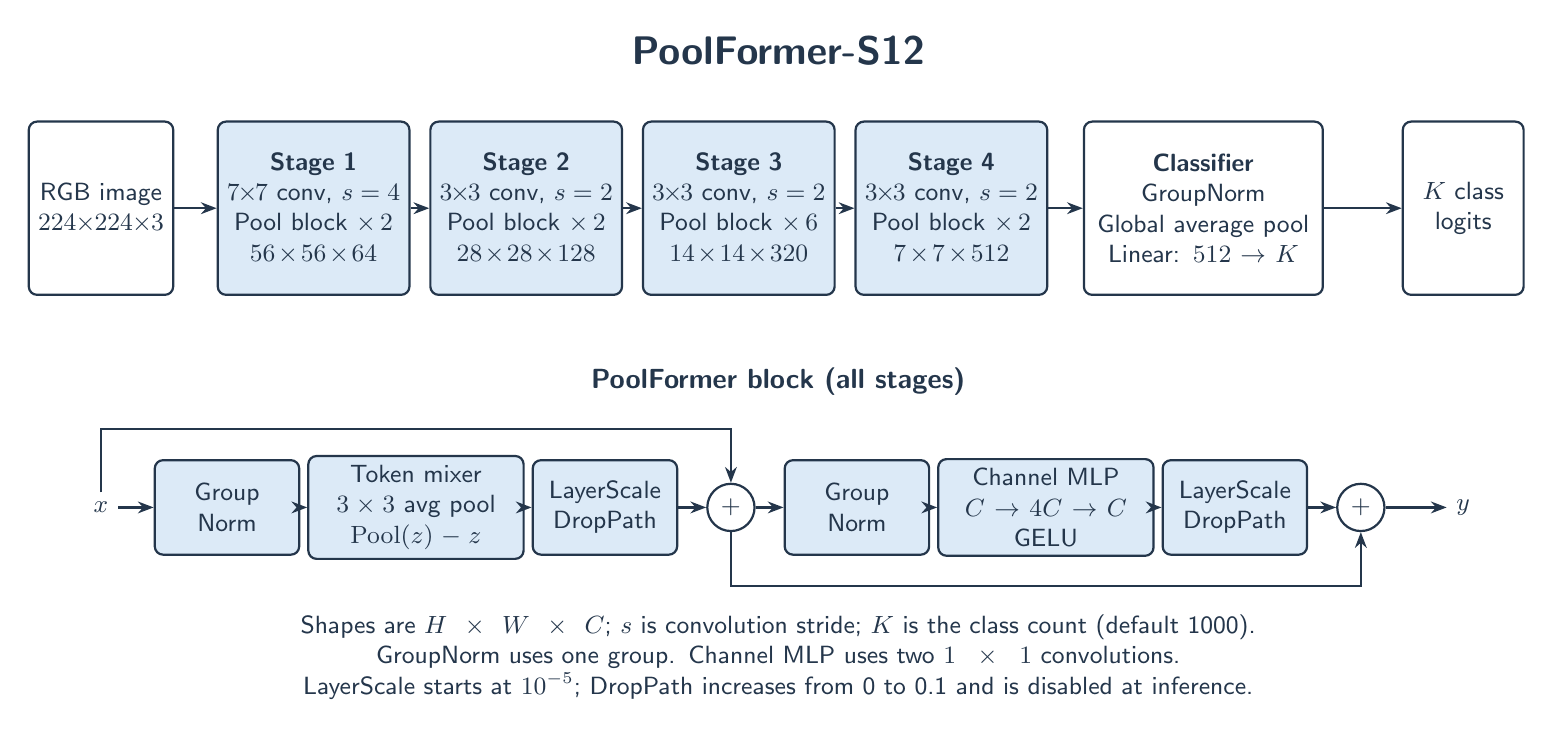
\begin{tikzpicture}[font=\sffamily\small,text=ink]
  \node[font=\sffamily\bfseries\Large] at (8.6,2) {PoolFormer-S12};
  \node[box,fill=white,text width=16mm] (input) at (0,0)
    {RGB image\\$224\!\times\!224\!\times\!3$};
  \node[box] (s1) at (2.7,0)
    {\textbf{Stage 1}\\$7\!\times\!7$ conv, $s=4$\\Pool block $\times\,2$\\$56\!\times\!56\!\times\!64$};
  \node[box] (s2) at (5.4,0)
    {\textbf{Stage 2}\\$3\!\times\!3$ conv, $s=2$\\Pool block $\times\,2$\\$28\!\times\!28\!\times\!128$};
  \node[box] (s3) at (8.1,0)
    {\textbf{Stage 3}\\$3\!\times\!3$ conv, $s=2$\\Pool block $\times\,6$\\$14\!\times\!14\!\times\!320$};
  \node[box] (s4) at (10.8,0)
    {\textbf{Stage 4}\\$3\!\times\!3$ conv, $s=2$\\Pool block $\times\,2$\\$7\!\times\!7\!\times\!512$};
  \node[box,fill=white,text width=28mm] (head) at (14,0)
    {\textbf{Classifier}\\GroupNorm\\Global average pool\\Linear: $512\to K$};
  \node[box,fill=white,text width=13mm] (output) at (17.3,0) {$K$ class\\logits};
  \draw[flow] (input) -- (s1);
  \draw[flow] (s1) -- (s2);
  \draw[flow] (s2) -- (s3);
  \draw[flow] (s3) -- (s4);
  \draw[flow] (s4) -- (head);
  \draw[flow] (head) -- (output);

  \node[font=\sffamily\bfseries] at (8.6,-2.2) {PoolFormer block (all stages)};
  \node (x) at (0,-3.8) {$x$};
  \node[op] (n1) at (1.6,-3.8) {Group\\Norm};
  \node[op,text width=25mm] (mix) at (4,-3.8)
    {Token mixer\\$3\times3$ avg pool\\$\operatorname{Pool}(z)-z$};
  \node[op] (ls1) at (6.4,-3.8) {LayerScale\\DropPath};
  \node[sum] (a1) at (8,-3.8) {$+$};
  \node[op] (n2) at (9.6,-3.8) {Group\\Norm};
  \node[op,text width=25mm] (mlp) at (12,-3.8)
    {Channel MLP\\$C\to4C\to C$\\GELU};
  \node[op] (ls2) at (14.4,-3.8) {LayerScale\\DropPath};
  \node[sum] (a2) at (16,-3.8) {$+$};
  \node (y) at (17.3,-3.8) {$y$};
  \draw[flow] (x) -- (n1);
  \draw[flow] (n1) -- (mix);
  \draw[flow] (mix) -- (ls1);
  \draw[flow] (ls1) -- (a1);
  \draw[flow] (a1) -- (n2);
  \draw[flow] (n2) -- (mlp);
  \draw[flow] (mlp) -- (ls2);
  \draw[flow] (ls2) -- (a2);
  \draw[flow] (a2) -- (y);
  \draw[flow] (x.north) -- (0,-2.8) -- (8,-2.8) -- (a1.north);
  \draw[flow] (a1.south) -- (8,-4.8) -- (16,-4.8) -- (a2.south);

  \node[align=center,text width=175mm] at (8.6,-5.7)
    {Shapes are $H\times W\times C$; $s$ is convolution stride; $K$ is the class count (default 1000).\\
     GroupNorm uses one group. Channel MLP uses two $1\times1$ convolutions.\\
     LayerScale starts at $10^{-5}$; DropPath increases from 0 to 0.1 and is disabled at inference.};
\end{tikzpicture}
\end{document}
